\documentclass[11pt,a4paper]{article}

\usepackage{graphicx, amsmath,amssymb,amsfonts, dsfont, hyperref, framed, enumitem,color}
\usepackage[left=2.5cm,right=2.5cm,top=3cm,bottom=3cm]{geometry}
\usepackage{listings}
\usepackage{floatrow}
\usepackage{subfig}
\usepackage{fancyhdr}
\usepackage{xcolor}
\usepackage{setspace}
\usepackage[font=small,labelfont=bf]{caption}
\linespread{1.2}
\renewcommand{\labelitemi}{$-$}
\pagestyle{fancy}
\fancyhf{}
\lhead{MATH3001}
\chead{Assessing flood mitigation policy using FEV}
\rhead{2018/2019}
\cfoot{\thepage}

\makeatletter 
\renewcommand\@biblabel[1]{#1.} 
\makeatother

\begin{document}
\floatsetup[figure]{style=plain,subcapbesideposition=top}

\begin{titlepage}
\begin{center}

\begin{figure}[t]
\raggedleft
\includegraphics[width=75mm]{Leeds_Logo.pdf}
\end{figure}
 

\vspace*{5cm}
{\huge \textbf{MATH3001: Project in Mathematics}}\\
\hrulefill

\vspace*{0.1cm}
{\LARGE Analysing five examples of extreme UK river floods and assessing flood mitigation policy, using flood-excess volume}\\
\vspace{1cm}
{\large Abbey Chapman}\\
{\large ID: 201005685 $|$ Supervisors: O. Bokhove and T. Kent}\\
\vfill
School of Mathematics\\
University of Leeds\\
2018/2019
\end{center}
\end{titlepage}

\tableofcontents 
\noindent \hrulefill

\newpage
\section{To do list}
\begin{itemize}
\item write report by monday
\item compile environement agency emails
\item send to mum for spell check
\item do graphs for leeds flood mitigation
\item do flood mitigation for avon - this is the main work yet to be done
\item make sure git hub is up to scratch
\item talk about supercritical and sub critical flows, github
\item affect of climate, could explain why it would be good to have flood mitigation above fev. include scholarly articles if possible.
\item check image referencing and no date
\item remove 2.3m from grr graph. talk about verage depth in text (i used when talking about grr longitudonal slope, 0.715m strat and 0.93 war.
\item talk about limits of automated code and what you would improve if you could continue.
\item order references
\item update tables
\item antonia verification
\end{itemize}

\newpage
\section{Introduction}
Major flooding events have had a huge detremental affect on the UKs' economy, its business and the community at large{;} ``In England and Wales alone, over 4 million people and properties valued at over £200 billion are at risk'' \cite{foresight} while the cost of the flooding across the UK on Boxing Day 2015 was estimated to have topped \pounds5 billion nationwide \cite{telegraph}. Thus, this project aims to use the analysis of flood data from the floods of a range of rivers and subsequently assess, by means of flood-excess volume, the cost efficacy of various proposed and hypothetical flood-mitigation policy with the aim of assisting policy makers, businesses and the general public in reducing the negative affects of floods. One way of achieving this, besides the creation of this report, is to produce an automated code that can produce a value for the flood-excess volume of any flood, thereby allowing policy makers and the general public to analyse floods using flood-excess volume which may be pertinent their interests or to investigate methods of mitigating, or even preventing, future flooding in their area.

Flood-excess volume can be simplisticly defined as the difference between the total volume of water discharged at a certain spatial location on a river during the time it is in flood and the maximum volume capacity of the river at this location when not in flood \cite{Aire}. This makes the flood-excess volume the volume of flood water that is actively causing flooding at that location on the river and therefore, by quantifying the volume of water a certain flood-mitigation policy reduces a flood by as well as the cost of implementing it, it is possible to to evaluate the percentage of flood-excess volume mitigated by said policy. The cost per percent of flood-excess volume mitigated of each policy can then be calculated and it is this method of analyzation that will be employed in this report.

To mitigate a flood is to reduce the amount of flooding, and thereby the damage as a result of such flooding, caused when a river breaks its banks. Flood-mitigation has been attempted since the very origins of non-nomadic humanity as the negative financial and social repercussions of a large flood (such as loss of property, crops, infrastructure and even life) are severe. Early examples of attempts to mitigate floods include the construction of stilt-houses by the Yue people in Ancient China around 7000 years ago \cite{yue}. In the modern world there are many different methods of flood-mitigation that can be used which include: Sustainable Urban Drainage Systems (SuDS), Natural Flood Management (NFM), the building of dams, high flood walls or barriers, river bed widening and the drawing down of drinking water reservoirs before predicted heavy rainfall. Each of these stated methods that will be further explored as part of this report.

As the integral work forming the basis of some sections in this report was performed as part of a team (comprised of A. Feilden, S. Kennet, M. Saunders, J. Willis and A. Chapman), an outline of the report is included below, hightlighting which sections were produced individually and which as part of the wider team.
\begin{framed}
\begin{itemize}
\item A review on the concept of flood-excess volume, introduced above, is performed in \S 2. This has been interperted individually by the author based on the work performed by O. Bokhove, T. Kent and M. Kelmanson in \cite{Aire} and \cite{Calder-Don}.
\item Analysis of the 2015 Boxing Day flooding of two rivers, the Rivers Aire in Leeds and Calder in Mytholmroyd, within the county of West Yorkshire is included in \S 3. This analysis includes calculation of flood-excess volume and based on this an assessment of various proposed flood-mitigation measures is performed. The original analysis and assessment was performed by the whole team, with the assistance of O. Bokhove and T. Kent.
\item \S 4 includes the same processes of analysis and assessment as \S 3 but for the 2007 floods along the River Don in Sheffield. Again, this was performed by the team.
\item The rest of the report includes analysis and assessment individually performed by the author. \S 5 includes the calculation of the flood-excess volume for the November 2012 floods along the River Avon, looking at two locations along the river{;} Stratford-upon-Avon and Warwick. Also included is the flood-excess volume calculated by A. Fielden as a verification of the authors results.
\item Having analysed flooding of the River Avon in \S 5, \S 6 contains assessment of both proposed and hypothetical flood-mitigation scenarios, using the flood-excess volumes calculated in \S 5.
\item A summary of the report is in \S 7 and conclusions from the report are drawn there. Acknowledgements and suggested further reading, including a web page created by the team giving instructions on how the geberal public can calculate the flood-excess volume for themselves, is also included here.
\end{itemize}
\end{framed}

\newpage
\section{Definition of flood-excess volume}
The flood-excess volume (henceforth abbreviated to FEV) is defined to be the volume of flood water that causes flooding at a specified location along a flooded river. FEV is therefore dependant on the threshold river level $h_T$. The definition of $h_T$ is the maximum level a river can reach without flooding{;} i.e. the river floods if the in situ river level $\overline{h}$ rises above $h_T$. The flow rate $Q$ is given from a pre determined rating curve which gives $Q$ as a function of $\overline{h}$. All the floods analysed as part of this report have the same equation relating $Q$ and $\overline{h}$
\begin{equation}\tag{2.1}
Q(\overline{h})=c_k (\overline{h}-a_k )^{b_k},\text{ }k=1,...,m,
\end{equation}
where the rating curve coefficients $a_k$, $b_k$ and $c_k$ are provided by the Environment Agency via email. The dimension of $a_k$ must be the same as the river level $\overline{h}$ it is being subtracted from, i.e. m$^3$. As $b_k$ is a power, it must be dimensionless which then forces $c_k$ to have dimension m$^{3-b_k}$/s in order for the dimension of the right side of the equation to match the dimention of the left, [$Q(\overline{h})$]= m$^3$/s. Each value of k corresponds to a range of $\overline{h}$ values, i.e. $h_{k-1}<\overline{h}<h_k$. During flooding events the maximum river level achieved is often higher than the upper bound of the last interval at which point the upper bound can be extrapolated to the maximum value of $\overline{h}$. As $\overline{h}=\overline{h}(t)$, the rating curve $Q=Q(\overline{h})$ means that the flow rate $Q$ can be found implicitly to be a function of time{;} $Q(\overline{h}(t))=Q(t)$.

\subsection{Approximations of the flood-excess volume}
FEV can be approximated using three different methods, each of varying accuracy. It should be noted that as the FEV is a volume it is in units of m$^3$. The total volume $V$ discharged by a river with flow rate $Q(\overline{h})$ over a given time interval can be approximated as
\begin{equation}\tag{2.1\textit{a}}
V\approx \sum_{i=1}^{n}(Q(\overline{h}_i))\Delta t,
\end{equation}
where n is the number of values for $Q(\overline{h})$ within the time interval and t is the time elapsed between each value of $Q(\overline{h})$. As the FEV ($V_e$) is defined as the excess volume discharged by the river once it has reach a level above $h_T$ until it is back below $h_T$, equation 2.1\textit{a} can easily be used to provide the best approximation for FEV
\begin{equation}\tag{2.1\textit{b}}
V_e\approx V_{e_1} = \sum_{i=1}^{n}(Q(\overline{h}_i)-Q_T)\Delta t,
\end{equation}
where $Q_T=Q(h_T)$ is constant as $h_T$ is a fixed value. In this case, n is the number of $Q(\overline{h})$ values from when the river level $\overline{h}$ goes above $h_T$ until it is back below $h_T$. The time that this takes is therefore the equivalent of the duration of the flood $T_f$. The time interval between subsequent $Q(\overline{h})$ values is thus $\Delta t=T_f/n$ and so as $n \to \infty$, $\Delta t \to 0$ this approximation becomes the exact area between the curve $Q(\overline{h})$ and the constant value $Q_T$, seen to be the shaded area inn Figure 1 b).

A second, less accurate, approximation of $V_e$ is given to be the area of the emboldened rectangle in Figure 1 b)
\begin{equation}\tag{2.1\textit{c}}
V_e \approx V_{e_2} = T_f(Q_m-Q_T),
\end{equation}
where $Q(h_m)=Q_m$ is the mean flow rate above $Q_T$. $Q_m$ can be found relatively accurately for each of the floods analysed by first finding the FEV using equation 2.1\textit{b} and then rearranging equation 2.1\textit{c} so that
\begin{equation}\tag{2.1\textit{d}}
Q_m\approx \frac{V_e}{T_f}+Q_T,
\end{equation}
from which $h_m$ is then found by rearranging equation 2.1.

The least accurate third approximation of $V_e$ is
\begin{equation}\tag{2.1\textit{e}}
V_e\approx V_{e_3}=(h_m-h_T)T_f\frac{Q_{max}}{h_{max}}
\end{equation}
which is found because $Q_m\approx (Q_{max}/h_{max})h_m$ and similarly $Q_T\approx (Q_{max}/h_{max})h_T$, approximation mostly used when there is no rating curve that explicitly gives $Q(\overline{h})$ \cite{Calder-Don}. $h_{max}$ and $Q_{max}$ stand for the maximum river level and flow rate value achieved during the period being analysed respectively. 

All FEVs calculated for the five floods analysed in this report have been calculated using the most accurate approximation, equation 2.1\textit{a}, given a $\Delta t$ of 15 minutes.

\newpage
\section{Verification; The Boxing Day 2015 floods in the county of West Yorkshire}
\subsection{The River Aire}
\begin{figure}[H]
\centering
\sidesubfloat[]{\includegraphics[scale=0.55]{Aire-Rainfall_Graph.png}}
\hfill
\sidesubfloat[]{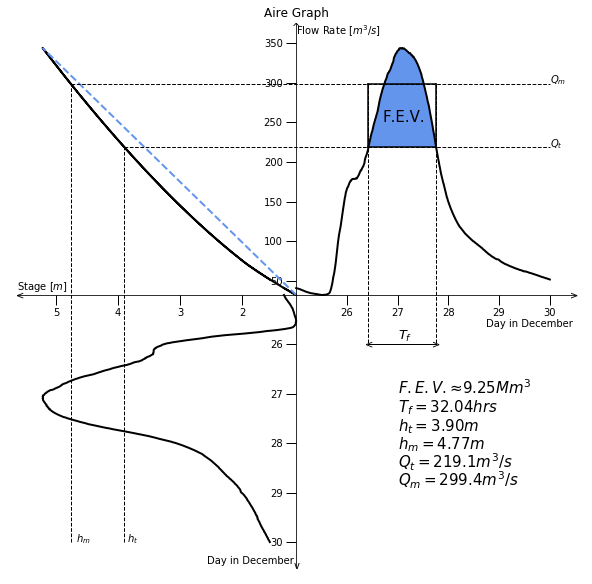
\includegraphics[scale=0.55]{Aire-Quadrant_Graph.png}}
\caption{Flow rate and river height data for the River Aire at the Armely gauging station in Leeds: a) river height ($\overline{h}$[m]) \cite{Aire} and catchment rainfall [mm] data \cite{NRFA} for a year starting from May 2015 (note, catchment rainfall data was not available for 2016) and b) quadrant plot for the 2015 Boxing Day floods of the River Aire. The top-left quadrant displays the rating curve (using data provided by Table 1) alongside its linear approximation (the blue dashed line), whilst the top-right and bottom-left quadrants display the river height ($\overline{h}$[m]) and flow rate ($Q$ [m$^3$/s]), respectively, during the floods. FEV is then the blue area below the flow rate curve (a function of $\overline{h}$, $Q(\overline{h})$, obtained from the rating curve) and above the flow rate corresponding to a given threshold height, $Q_T =Q(h_T)$. $\overline{h}=\overline{h}(t)$, where t is the number of days after the 25\textsuperscript{th} of December 2015, meaning $Q(\overline{h})=Q(t)$. Equation 2.1\textit{a} is applied to provide $V_e \approx V_{e_1}$= 9.34Mm$^3$, the blue shaded area. The emboldened rectangle approximates the FEV using equation 2.1\textit{c} so that $V_{e_2}= (Q_m -Q_T )\cdot T_f \approx V_{e_1}$= 9.34Mm$^3$, thereby providing an approximation of $Q_m$ given fixed $Q_T$=219.1m$^3$/s and calculated $T_f$=32 hours. Rearranging the rating curve equation 2.1 will provide an evaluation of $h_m$=4.77m from $Q_m$.}
\end{figure}

\begin{table}[H]
\centering
\begin{tabular}{l|l|l|l|l|l}
$k$ & $h_{k-1}$ [m] & $h_k$ [m] & $c_k$ [m$^{3-b_k}$/s] & $b_k$ [-] & $a_k$ [m]\\
\hline
1 & 0.2 & 0.685 & 30.69 & 1.115 & 0.156 \\
2 & 0.685 & 1.917 & 27.884 & 1.462 & 0.028 \\
3 & 1.917 & 4.17 & 30.127 & 1.502 & 0.153 \\
\end{tabular}
\caption{The coefficients $a_k$, $b_k$ and $c_k$ and their corresponding upper ($h_k$) and lower ($h_{k-1}$) bounds on $\overline{h}$ \cite{Aire} applied in the calculation of the rating curve, using equation 2.1, at the Armley gauging station on the River Aire.}
\end{table}

\subsubsection{Past and planned mitigation projects in Leeds}

\subsection{The River Calder}

\begin{figure}[H]
\centering
\sidesubfloat[]{\includegraphics[scale=0.55]{Calder-Rainfall_Graph.png}}
\hfill
\sidesubfloat[]{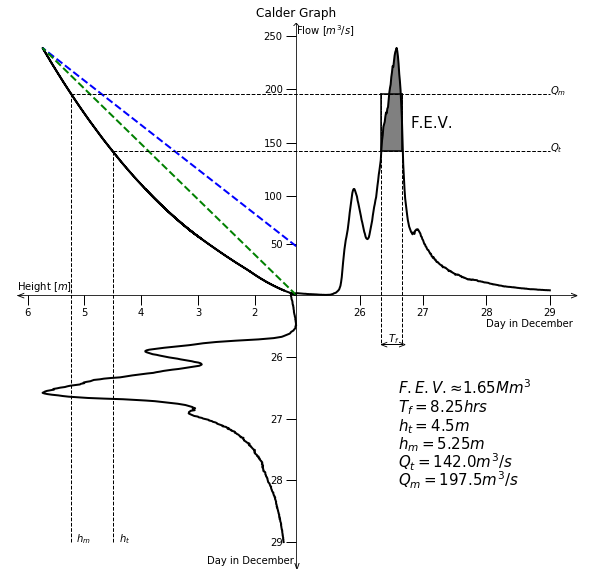
\includegraphics[scale=0.55]{Calder-Quadrant_Graph.png}}
\caption{Flow rate and river height data for the River Calder at the Mytholmroyd gauging station: a) river height ($\overline{h}$[m]) \cite{Calder-Don} and catchment rainfall [mm] data \cite{NRFA} for a year starting from May 2015 (note, catchment rainfall data was not available for 2016) and b) quadrant plot for the 2015 Boxing Day floods of the River Calder (\textit{cf.} Figure 1 b)).}
\end{figure}

\begin{table}[H]
\centering
\begin{tabular}{l|l|l|l|l|l}
$k$ & $h_{k-1}$ [m] & $h_k$ [m] & $c_k$ [m$^{3-b_k}$/s] & $b_k$ [-] & $a_k$ [m]\\
\hline
1 & 0 & 2.107 & 8.459 & 2.239 & 0.342 \\
2 & 2.107 & 3.088 & 21.5 & 1.37 & 0.826 \\
3 & 3.088 & 5.8 & 2.086 & 2.515 & -0.856 \\
\end{tabular}
\caption{The coefficients $a_k$, $b_k$ and $c_k$ and their corresponding upper ($h_k$) and lower ($h_{k-1}$) bounds on $\overline{h}$ \cite{Calder-Don} applied in the calculation of the rating curve, using equation 2.1, at the Mythomroyd gauging station on the River Calder.}
\end{table}

\subsubsection{Past and planned mitigation projects in Calderdale}

\newpage
\section{Verification; The June 2007 flood of the River Don}
\begin{figure}[H]
\centering
\sidesubfloat[]{\includegraphics[scale=0.55]{Don-Rainfall_Graph.png}}
\hfill
\sidesubfloat[]{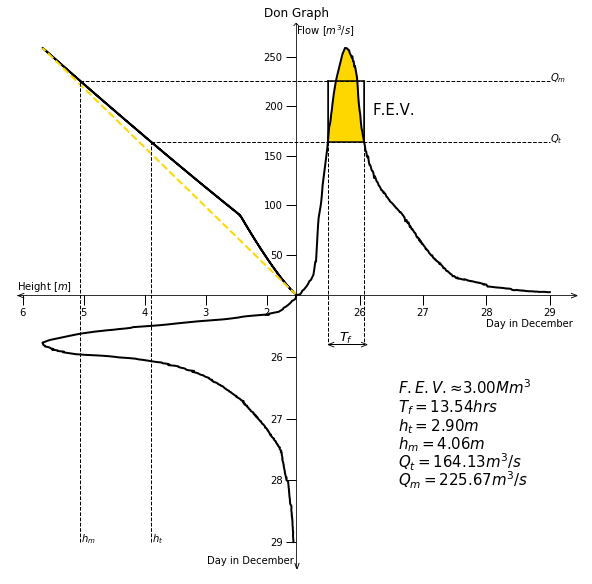
\includegraphics[scale=0.55]{Don-Quadrant_Graph.png}}
\caption{Flow rate and river height data for the River Don at the Sheffield Hadfields: a) river height ($\overline{h}$[m]) \cite{Calder-Don} and catchment rainfall [mm] data \cite{NRFA} for a year starting from January 2007 and b) quadrant plot for the June 2007 floods of the River Don (\textit{cf.} Figure 1 b)), where the time values in this case give the number of days after the 25\textsuperscript{th} of June 2007.}
\end{figure}

\begin{table}[H]
\centering
\begin{tabular}{l|l|l|l|l|l}
$k$ & $h_{k-1}$ [m] & $h_k$ [m] & $c_k$ [m$^{3-b_k}$/s] & $b_k$ [-] & $a_k$ [m]\\
\hline
1 & 0 & 0.52 & 78.4407 & 1.7742 & 0.223 \\
2 & 0.52 & 0.931 & 77.2829 & 1.3803 & 0.3077 \\
3 & 0.931 & 1.436 & 79.5956 & 1.2967 & 0.34 \\
4 & 1.436 & 3.58 & 41.3367 & 1.1066 & -0.5767 \\
\end{tabular}
\caption{The coefficients $a_k$, $b_k$ and $c_k$ and their corresponding upper ($h_k$) and lower ($h_{k-1}$) bounds on $\overline{h}$ \cite{Calder-Don} applied in the calculation of the rating curve, using equation 2.1, at the Sheffield Hadfields gauging station on the River Don.}
\end{table}

\subsection{Past and planned mitigation projects in Sheffield}

\newpage
\section{The November 2012 flood of the River Avon}
\begin{figure}[H]
\centering
\subfloat{\includegraphics[scale=0.2]{Stratford-Flooding-Plaque.png}}
\subfloat{\includegraphics[scale=0.4]{Stratford-Flooded.jpg}}
\hfill
\subfloat{\includegraphics[scale=0.229]{Warwick-Castle.png}}
\subfloat{\includegraphics[scale=0.203]{Warwick-Castle-Flooded.png}}
\caption{Flooding in Stratford-upon-Avon and Warwick: the top left photo is of a plaque in Stratford-upon-Avon displaying historic flood height highs{;} it was erected before the 2012 flooding event \cite{plaque}. The top right is a photo of Bancfrotft in Stratford-upon-Avon during a flood \cite{strat-flood}. The bottom two photos are of the famous Warwick Castle, the left \cite{castle} unflooded and the right \cite{warwick-flooding} during a flood. The gauging stations in both Warwick and Stratford-upon-Avon are very slightly upstream from the Castle and Bancroft respectively meaning it is these areas of flooding that will be analysed.}
\end{figure}


\subsection{The flood in Stratford-upon-Avon}
\begin{figure}[H]
\centering
\sidesubfloat[]{\includegraphics[scale=0.55]{Stratford-Rainfall_Graph.png}}
\hfill
\sidesubfloat[]{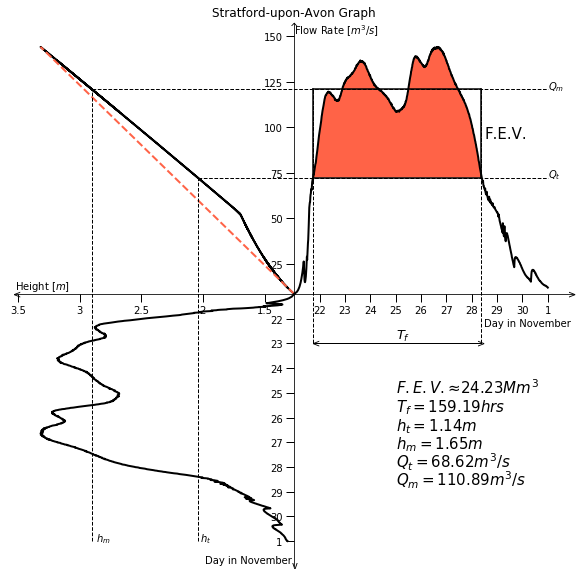
\includegraphics[scale=0.55]{Stratford-Quadrant_Graph.png}}
\caption{Flow rate and river height for the River Avon at the Cox's Yard gauging station in Stratford-upon-Avon: a) river height ($\overline{h}$[m]) \cite{EA} and catchment rainfall [mm] data \cite{NRFA} for the months of November and December 2012 (note, catchment rainfall data was not available for this gauging station so data was instead obtained for the next nearest geographical station, Alscot Park on the River Stour) and b) quadrant plot for the November 2012 floods of the River Avon at Stratford-upon-Avon (\textit{cf.} Figure 1 b)), where the time values in this case are the number of days from the 21\textsuperscript{st} of November 2012.}
\end{figure}

\begin{table}[H]
\begin{tabular}{l|l|l|l|l|l}
$k$ & $h_{k-1}$ [m] & $h_k$ [m] & $c_k$ [m$^{3-b_k}$/s] & $b_k$ [-] & $a_k$ [m]\\
\hline
1 & 0.136 & 0.938 & 158.04 & 2.85438 & 0.262919 \\
2 & 0.938 & 1.427 & 87.0362 & 0.962129 & 0.358741 \\
\end{tabular}
\caption{The coefficients $a_k$, $b_k$ and $c_k$ and their corresponding upper ($h_k$) and lower ($h_{k-1}$) bounds on $\overline{h}$ \cite{EA} applied in the calculation of the rating curve, using equation 2.1, at the Cox's Yard gauging station on the River Avon.}
\end{table}

\begin{figure}[H]
\centering
\subfloat[]{\includegraphics[scale=0.55]{Stratford-FEV_ht_Graph.png}}
\hfill
\subfloat[]{\includegraphics[scale=0.6]{Stratford-Square_Lake_Graph.png}}
\subfloat[]{\includegraphics[scale=0.4]{Stratford-Adding_FEV_Graph.png}}
\caption{Stratford-upon-Avon square lake graphs for the November 2012 flood: a) is a visual aid demonstrating the relationship between a chosen $h_T$ and both its corresponding FEV (the red line with crosses) and square lake side length (the light blue line with circles) where b) demonstrates what is meant by square lake side length, the side length of our calculated FEV's (1.83Mm$^3$) 2m deep square lake being 956.56m. c) shows how the calculated FEV (\textit{cf.} Figure 1 b)) for the seperated peaks (the middle peak corresponds to the green line with triangles, the right peak to the blue line with circles and the leftmost peak, which then disapears above $h_T$ = 1.6m, to the black square) of $Q(t)$ above $Q_T$ (as seen in Figure 4 b)) is then added together to approximate the total FEV (the red line with crosses).}
\end{figure}

\subsubsection{Verification of the Stratford-upon-Avon FEV of November 2012}

\subsection{The flood in Warwick}
\begin{figure}[H]
\centering
\sidesubfloat[]{\includegraphics[scale=0.55]{Warwick-Rainfall_Graph.png}}
\hfill
\sidesubfloat[]{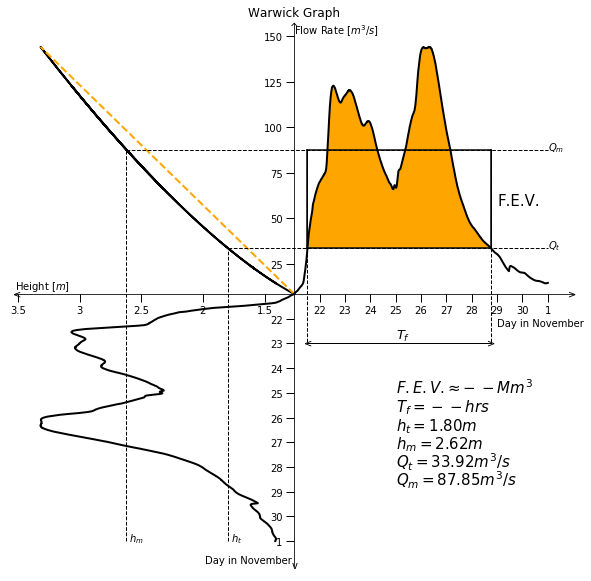
\includegraphics[scale=0.55]{Warwick-Quadrant_Graph.png}}
\caption{Flow rate and river height for the River Avon at the Warwick gauging station: a) river height ($\overline{h}$[m]) \cite{EA} and catchment rainfall [mm] data \cite{NRFA} for the months of November and December 2012. b) quadrant plot for the November 2012 floods of the River Avon at Warwick (\textit{cf.} Figure 1 b)), where the time values in this case are the number of days from the 21\textsuperscript{st} of November 2012.}
\end{figure}

\begin{table}[H]
\centering
\begin{tabular}{l|l|l|l|l|l}
$k$ & $h_{k-1}$ [m] & $h_k$ [m] & $c_k$ [m$^{3-b_k}$/s] & $b_k$ [-] & $a_k$ [m]\\
\hline
1 & 0.960 & 3.000 & 40.6178 & 1.44854 & 0.917837 \\
\end{tabular}
\caption{The coefficients $a_k$, $b_k$ and $c_k$ and their corresponding upper ($h_k$) and lower ($h_{k-1}$) bounds on $\overline{h}$ \cite{EA} applied in the calculation of the rating curve, using equation 2.1, at the Warwick gauging station on the River Avon.}
\end{table}

\begin{figure}[H]
\centering
\subfloat[]{\includegraphics[scale=0.55]{Warwick-FEV_ht_Graph.png}}
\hfill
\subfloat[]{\includegraphics[scale=0.6]{Warwick-Square_Lake_Graph.png}}
\subfloat[]{\includegraphics[scale=0.4]{Warwick-Adding_FEV_Graph.png}}
\caption{Warwick square lake graphs for the November 2012 flood: a) is a visual aid demonstrating the relationship between a chosen $h_T$ and both its corresponding FEV (the orange line with crosses) and square lake side length (the light blue line with circles) where b) demonstrates what is meant by square lake side length, the side length of our calculated FEV's (0.74Mm$^3$) 2m deep square lake being 908.28m. c) gives the individual FEV of seperated peaks when they occur {;}the leftmost peak corresponds to the black line with squares, the right peak to the blue line with circles and the middle peak, when it does exist, to the green triangles (\textit{cf.} Figure 6 c)). The total FEV is given by the orange line with crosses.}
\end{figure}

\subsubsection{Verification of the Warwick FEV of November 2012}

\newpage
\section{Flood-mitigation assessment using FEV}
\begin{figure}[H]
\begin{center}
\subfloat{\includegraphics[scale=0.5]{Stratford-Warwick-Flood_Risk_Map.png}}
\caption{Flood-risk map for the stretch of the River Avon in between Warwick and Stratford-upon-Avon \cite{flood-risk}. The location of the gauging stations in Warwick and Stratford-upon-Avon are given by the orange and red markers repectively. St. John's brook is denoted by the pink marker, Charlecote park by the green marker and the Racecourse brook by the yellow marker{;} each of which could potentially provide extra flood water storage. \textbf{could include river bed widening just after warwick castle, new map?}}
\end{center}
\end{figure}

\subsection{Past and planned mitigation projects upstream of Stratford-upon-Avon}

\subsection{Sustainable urban drainage systems (SuDS)}

\subsection{Natural flood management}

\subsubsection{Flow-attenuation features}

\subsubsection{Tree planting}

\subsection{Storage of flood water in reservoirs}

\subsection{Giving room to the River}

\begin{figure}[!ht]
\sidesubfloat[]{\includegraphics[scale=0.45]{GRR-1.png}}
\hfill
\sidesubfloat[]{\includegraphics[scale=0.45]{GRR-2.png}}
\caption{Very simple transverse profiles of the River Avon: a) shows the profile as it is now, with and average height of 2.3m and and average width of 3.96m \cite{canal}, whilst b) gives the approximated profile once the river bed has been widened, by 1m at a height above the river bed of 2m, as part of the giving room to the river process. The gradient of the new slope (1/b) is approximately the same as before the process.}
\end{figure}

\newpage
\section{Summary and discussion}

\subsection{Futher Reading}
The main source of information in regards to the flood-excess volume analysis used in this report was provided from the two articles \cite{Aire} and \cite{Calder-Don}, co-authored by the supervisors of this project, O. Bokhove and T. Kent. As such it would be beneficial to read these articles if there is a wish gain a broader understanding of the subject. Detailed information on the various methods of NFM is provided by the Environment Agency in \cite{nfm}. More information on what may happen in the future in regards to flood management nation wide is included \cite{foresight}, produced by the Flood and Coastal Defence project of the Foresight programme.

As part of this project the author, with the assistance of A. Feliden, S. Kennet, M. Saunder and J. Willis, has created a web page containing all the instruction need to perform the same FEV analysis as in this report. This includes as automated code, written by the author, which only needs the parameters of the rating curve and a chose $h_T$ to produce a graph and provide an evaluation of the FEV, $Q_m$, $Q_T$, $h_m$ and $T_f$. The code and the graph it produces may be found in the Appendix. There are some limits to the automated nature of this code, such as the fact that if the curve $Q(\overline{h})$ is split into more than one peak above $Q_T$ then, although the FEV calculated will be accurate, $T_f$ and thereby $Q_m$ and $h_m$ will not. The code also will not work if the flood data being analysed does not cover an integer number of days. Therefore, if this project were to be continued, fixing these issues would be strived for. 

\subsection{Acknowledgements}
The author would like to thank and acknowledge the Environment Agency in the West Midlands for contributing river height and flow rate data for the Warwick and Cox's Yard gauging stations, alongside each stations rating curve information, towards this report. This report Contains public sector information licensed under the Open Government Licence v3.0.

\newpage
\section{References}
\begin{thebibliography}{}
\bibitem{foresight}
Flood and Coastal Defence Project of the Foresight programme. \textit{Foresight: Future Flooding}. [Online]. 2004. [Accessed 14 March 2019]. Available from: https://assets.publishing.service.gov.uk/

\bibitem{telegraph}
Burn-Callander, R. \textit{UK flooding: cost of damage to top £5bn but many homes and businesses underinsured}. [Online]. 2015. [Accessed 14 March 2019]. Available from: https://www.telegraph.co.uk/

\bibitem{yue}
Peters, H. \textit{Tattooed Faces and Stilt Houses: Who Were the Ancient Yue?}. [Online]. 1990. [Accessed 14 March 2019]. Available from: http://sino-platonic.org/

\bibitem{}
Warwickshire County Council. \textit{Surface Water Management Plan Methodology Report}. [Online]. 2015. [Accessed 14 March 2019]. Available from: https://apps.warwickshire.gov.uk/

\bibitem{}
Warwickshire County Council. \textit{Local Flood Risk Management Strategy}. [Online]. 2016. [Accessed 14 March 2019]. Available from: https://apps.warwickshire.gov.uk/

\bibitem{}
GaugeMap. \textit{Stratford (River Avon), Warwick (River Avon)}. [Online]. 2019. [Accessed 14 March 2019]. Available from: https://www.gaugemap.co.uk/

\bibitem{}
BBC News \textit{Warwickshire floods: Three swept away in car escape injury}. [Online]. 2012. [Accessed 14 March 2019]. Available from: https://www.bbc.co.uk/

\bibitem{castle}
Brown, E. \textit{Warwick Castle - River Avon, Warwick}. [Online]. 2016. [Accessed 14 March 2019]. Available from: https://www.flickr.com/

\bibitem{warwick-flooding}
Dimmer, S. \textit{Flood alerts issued for parts of Warwickshire}. [Online]. 2015. [Accessed 14 March 2019]. Available from: https://www.coventrytelegraph.net/

\bibitem{brook}
English Severn \& Wye. \textit{Regional Flood Coastal Committee: Tuesday 8 January 2019 agenda}. [Online]. 2019. [Accessed 14 March 2019]. Available from: https://assets.publishing.service.gov.uk/

\bibitem{recent-high}
River Levels. \textit{River Avon at Stratford}. [Online]. 2019. [Accessed 14 March 2019]. Available from: https://riverlevels.uk/

\bibitem{plaque}
Smith, C. \textit{Updated: River Avon remains on flood alert despite falling water levels}. [Online]. 2018. [Accessed 14 March 2019]. Available from: http://www.stratford-herald.com/

\bibitem{canal}
UK Waterways Guide. \textit{A brief history of the River Avon}. [Online]. 2019. [Accessed 14 March 2019]. Available from: https://www.ukwaterwaysguide.co.uk/

\bibitem{}
susdrain. \textit{Stroud Rural Suds, Stroud}. [Online]. 2018. [Accessed 14 March 2019]. Available from: https://www.susdrain.org/

\bibitem{}
Woodland Trust. \textit{Natural flood management guidance: Woody dams, deflectors and diverters}. [Online]. 2016. [Accessed 14 March 2019]. Available from: https://www.woodlandtrust.org.uk/

\bibitem{leaky-dams}
Rural Payments Agency and Natural England. \textit{RP33: Large leaky woody dams}. [Online]. 2017. [Accessed 14 March 2019]. Available from: https://www.gov.uk/

\bibitem{ht}
Flood information service. \textit{River level: River Avon at Stratford}. [Online]. 2019. [Accessed 14 March 2019]. Available from: https://flood-warning-information.service.gov.uk/

\bibitem{Aire}
Bokhove, O., Kelmanson, M. and Kent, T. \textit{On using flood-excess volume in flood mitigation, exemplified for the River Aire Boxing Day Flood of 2015}. [Online]. 2018. [Accessed 14 March 2019]. Available from: https://eartharxiv.org/

\bibitem{NRFA}
National River Flow Archive. \textit{NERC CEH, Warwick, Armely, Mytholmroyd, Sheffield Hadfields, Alscot Park}. [Online]. 2019. [Accessed 14 March 2019]. Available from: https://nrfa.ceh.ac.uk/

\bibitem{}
Environment Agency. \textit{Natural flood management – part of the nation’s flood resilience}. [Online]. 2017. [Accessed 14 March 2019]. Available from: https://www.gov.uk/

\bibitem{suds}
Bayon, J., Charlesworth, S., Jato-Espino and Warwick, F. Rainfall–Runoff Simulations to Assess the Potential of SuDS for Mitigating Flooding in Highly Urbanized Catchments. \textit{International Journal of Environmental Research and Public Health}. 2016, \textbf{13}(1), 149.

\bibitem{flood-risk}
Environment Agency. \textit{Likelihood of flooding in this area}. [Online]. 2017. [Accessed 14 March 2019]. Available from: https://flood-map-for-planning.service.gov.uk/

\bibitem{Calder-Don}
Bokhove, O., Kelmanson, M. and Kent, T. \textit{On using flood-excess volume to assess natural flood management, exemplified for extreme 2007 and 2015 floods in Yorkshire}. [Online]. 2018. [Accessed 14 March 2019]. Available from: https://eartharxiv.org/

\bibitem{EA}
Weston, M. on behalf of the Environment Agency in the West Midlands. \textit{Email to Abbey Chapman}. 20 November, 2018.

\bibitem{strat-flood}
Lugg, B. \textit{New emergency flood barrier tested in Stratford}. [Online]. 2017. [Accessed 15 March 2019]. Available from: http://www.stratford-herald.com/

\bibitem{grr}
Environment Agency. \textit{Cost estimation for channel management}. [Online]. 2015. [Accessed 14 March 2019]. Available from: http://evidence.environment-agency.gov.uk/

\bibitem{flood-gate}
Environment Agency. \textit{Cost estimation for control assets}. [Online]. 2015. [Accessed 15 March 2019]. Available from: http://evidence.environment-agency.gov.uk/

\bibitem{drainage-area}
The Editors of Encyclopedia Britannica. \textit{River Avon}. [Online]. 2014. [Accessed 15 March 2019]. Available from:  https://www.britannica.com/

\bibitem{trees}
Natural England. \textit{Countryside Stewardship Manual: Woodland Creation Grant}. [Online]. 2018. [Accessed 15 March 2019]. Available from: https://assets.publishing.service.gov.uk/

\bibitem{altitude}
Route Calculator. \textit{Altitude Stratford-upon-Avon, Warwick, UK}. [Online]. \textbf{no date}. [Accessed 16 March 2019]. Available from: https://routecalculator.co.uk/

\bibitem{crow}
Doogal. \textit{Measuring distances}. [Online]. \textbf{no date}. [Accessed 16 March 2019]. Available from: https://www.doogal.co.uk/

\bibitem{n}
FishXing. \textit{Manning's n Values}. [Online]. 2006. [Accessed 16 March 2019]. Available from: http://www.fsl.orst.edu/

\bibitem{manning}
Okiishi, T., Musnon, B. and Young, D. \textit{Fundamentals of Fluid Mechanics}. [Online]. . [Accessed 16 March 2019]. Available from: 

\bibitem{nfm}
Environment Agency. \textit{Working with Natural Processes - Evidence Directory}. [Online]. 2018. [Accessed 16 March 2019]. Available from: https://assets.publishing.service.gov.uk/
\bibitem{}
. \textit{}. [Online]. . [Accessed 16 March 2019]. Available from:

\bibitem{}
. \textit{}. [Online]. . [Accessed 16 March 2019]. Available from:

\bibitem{}
. \textit{}. [Online]. . [Accessed 16 March 2019]. Available from:

\bibitem{}
. \textit{}. [Online]. . [Accessed 16 March 2019]. Available from:
\end{thebibliography}


\newpage
\appendix
\section{Appendix}
{\bf The graph that the automated FEV code produces using the example of the 2015 Boxing Day flood of the River Aire at Armley as an example}\\
\begin{figure}[H]
\begin{center}
\subfloat{\includegraphics[scale=0.55]{Automated-Aire_Example.png}}
\end{center}
\end{figure}
{\bf The automated FEV code- written in the python coding language}\\
\begin{spacing}{1}\footnotesize{\lstinputlisting[language=Python]{Automated-Quadrant-Graph-Code.py}}
\end{spacing}


\end{document}
